
\chapter{Results}

%COFs with high conformational degrees of freedom (like alkyl chain) were purposely excluded from the set since they are not well suited for the type of calculations performed here and should be treated differently using a different approach.


\section{Preliminary tests}
All preliminary test were performed by establishing the potential along the z axis on COF1 without x and y offsets between the sheets.

\subsection{Lennard-Jones}
Since the Lennard-Jones potential was implemented as a built-in function and not using an established program, a benchmarking was performed using the Lennard-Jones implementation of LAMMPS as a reference. The results are displayed on Figure \ref{fig:lj_bench}

\begin{figure}%[H]
\centering
\begin{tabular}{cr}
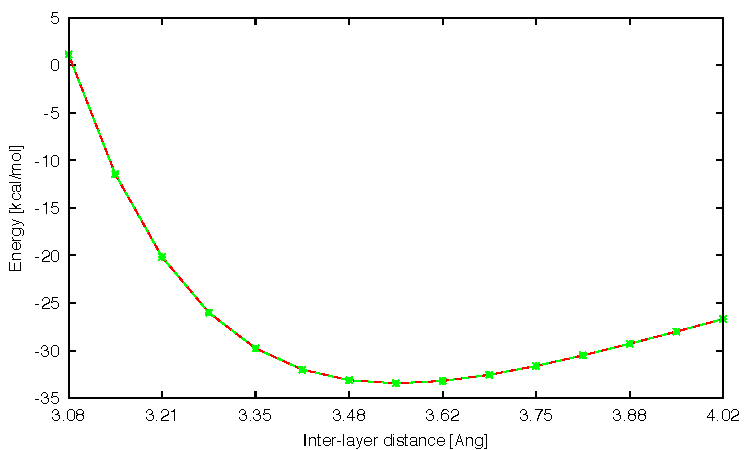
\includegraphics[width=6cm]{images/bench_lj.pdf}&  
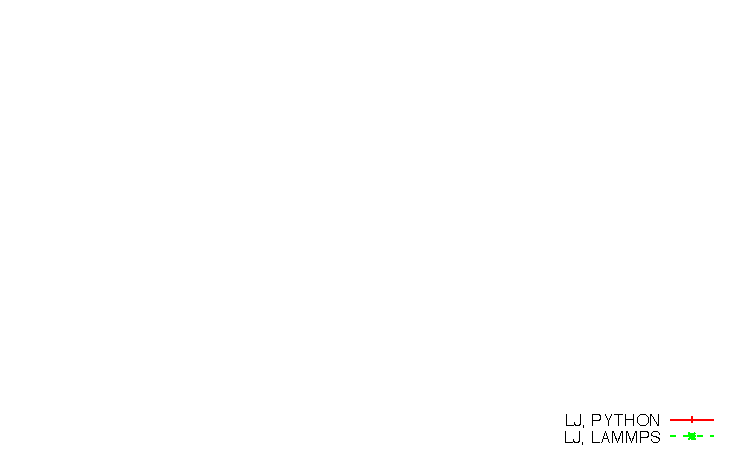
\includegraphics{images/key_bench_lj.pdf}\\
\end{tabular}
\caption{Comparison of the Lennard-Jones potential computed using our program and LAMMPS using a cutoff of 15$\AA$  and no tail correction}
\label{fig:lj_bench}
\end{figure}

The conclusion was that the Lennard-Jones potential was correctly implemented in the algorithm.




\begin{samepage}


Then a convergence test was performed to estimate the necessary cutoff. The potential obtained using different cutoffs are displayed on Figure \ref{fig:LJ_conv}

\begin{figure}[H]
\centering
\begin{tabular}{cr}
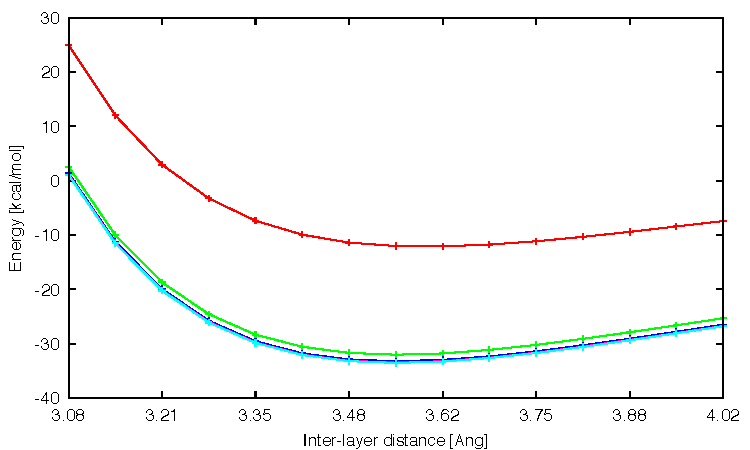
\includegraphics[width=6cm]{images/LJ_conv.pdf}& 
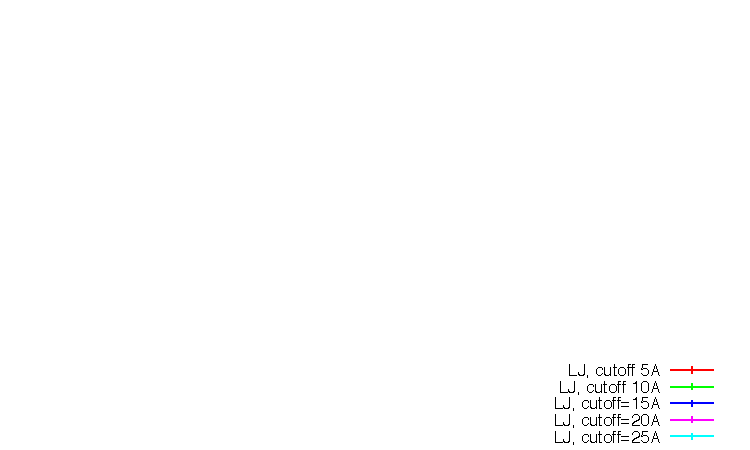
\includegraphics{images/key_lj.pdf} \\
\end{tabular}
\caption{Comparison of the Lennard-Jones potential as a function of the cutoff in $\AA$}
\label{fig:LJ_conv}
\end{figure}

From this, the conclusion was that a cutoff of 15 $\AA$ was sufficient.
\end{samepage}


\begin{samepage}

\subsection{Coulombic interactions}

As a first attempt, the coulombic interaction was also implemented as a built-in function with different tail corrections and damping functions, the Ewald summation implemented on LAMMPS was used as the reference. The results are displayed on Figure \ref{fig:coul_conv}

\begin{figure}[H]
\centering
\begin{tabular}{cr}
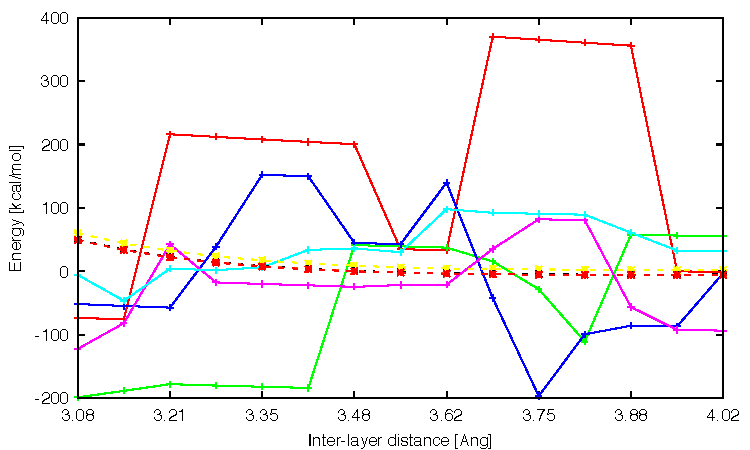
\includegraphics[width=6cm]{images/Coul_conv.pdf}&
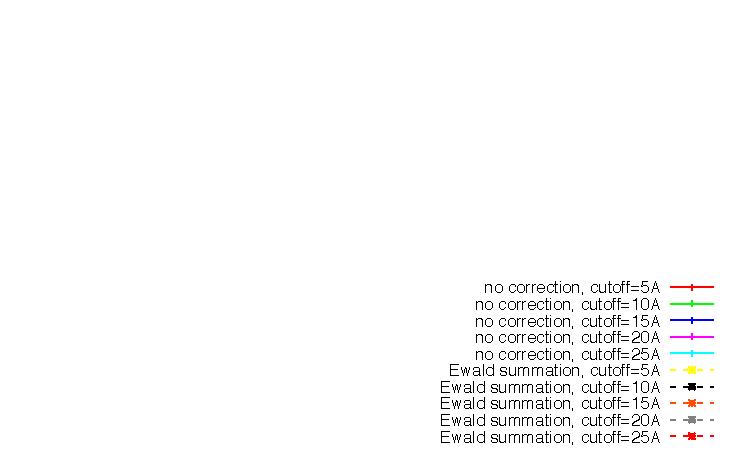
\includegraphics{images/key.pdf} \\
\end{tabular}
\caption{Comparison of the coulombic potentials with and without correction.}
\label{fig:coul_conv}
\end{figure}

\end{samepage}

\section{Stacking assessment and PESs}
\begin{figure}%[H]
\centering
\begin{tabular}{|c||c|c|c|c|c|c|}
\hline
COF & axis & LJ & LJ+Coul. & xTB & DFTB+ & DFT\\
\hline
\hline
\multirow{3}{*}[-0.3cm]{05000N2}&x&-1.88&-16.28&$/^*$&-2.50&-4.06\\
\cline{2-7}
&y&-8.68&8.68&$/^*$&0&-3.02\\
\cline{2-7}
&z&3.22&3.15&$/^*$&2.95&3.63\\
\hline
\hline
\multirow{3}{*}[-0.3cm]{05001N2}&x&3.00&-1.19&$/^*$&-1.19&-2.43\\
\cline{2-7}
&y&8.23&6.17&$/^*$&-2.06&-4.20\\
\cline{2-7}
&z&3.32&3.39&$/^*$&2.98&3.42\\
\hline
\hline
\multirow{3}{*}[-0.3cm]{10000N2}&x&0.73&2.94&-0.73&0&-3.88\\
\cline{2-7}
&y&-1.27&-2.54&-3.82&2.54&2.79\\
\cline{2-7}
&z&3.43&3.42&3.23&3.02&3.43\\
\hline
\hline
\multirow{3}{*}[-0.3cm]{13000N2}&x&-1.75&-13.41&15.74&-13.99&-12.41\\
\cline{2-7}
&y&-1.01&11.12&-9.09&8.08&9.68\\
\cline{2-7}
&z&3.40&3.13&2.93&3.00&3.05\\
\hline
\hline
\multirow{3}{*}[-0.3cm]{17120N2}&x&8.63&-11.09&-0.62&-0.62&-0.15\\
\cline{2-7}
&y&-4.27&-4.27&9.61&9.61&4.52\\
\cline{2-7}
&z&4.37&4.37&3.95&3.95&4.38\\
\hline
\hline
\multirow{3}{*}[-0.3cm]{18112N2}&x&0&0&0&0&0.19\\
\cline{2-7}
&y&0&0&0&0&0.11\\
\cline{2-7}
&z&4.04&4.04&3.82&3.89&9.92\\
\hline
\end{tabular}

\caption{Optimal offset found for each COF and for each technique given as an x,y,z vector in $\AA$.} 
\label{fig:overview}
\end{figure}

\let\thefootnote\relax\footnote{ $/^*$ see section \ref{sec:xTB_fail}}



%\cite{pizzi_aiida:_2016}




\begin{figure}[H]
\vspace{2cm}
\begin{centering}
\textbf{\LARGE{05000N2}}\par\medskip
\end{centering}
\makebox[\textwidth][c]{
\begin{tabular}{cc}
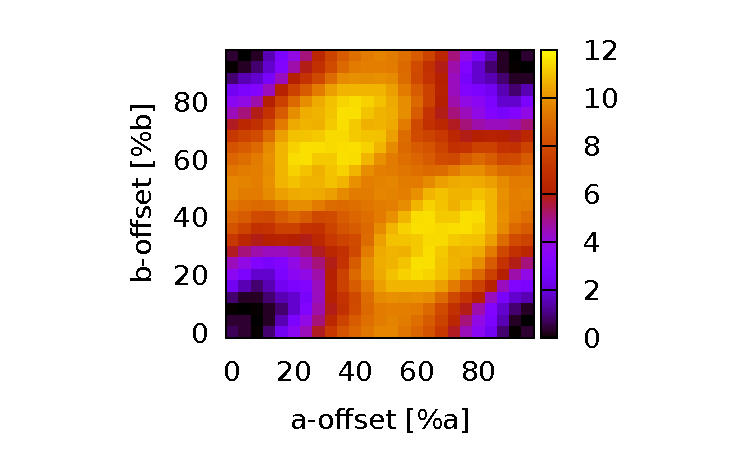
\includegraphics[trim={2cm 0cm 1.9cm 0.4cm},clip,width=8.5cm]{images/LJ_all_05000N2_map.pdf}& 
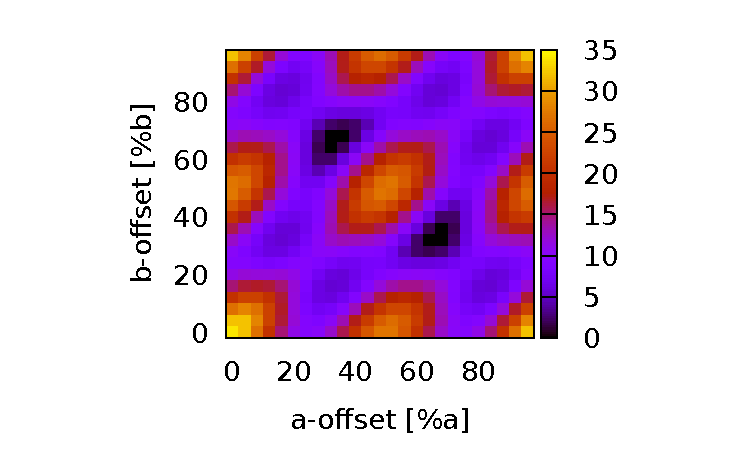
\includegraphics[trim={2cm 0cm 1.9cm 0.4cm},clip,width=8.5cm]{images/LAMMPS_all_05000N2_map.pdf}\\
\textbf{\Large{LJ}}\par\medskip & \textbf{\Large{LJ+Coul.}}\par\medskip\\
\multicolumn{2}{c}{ 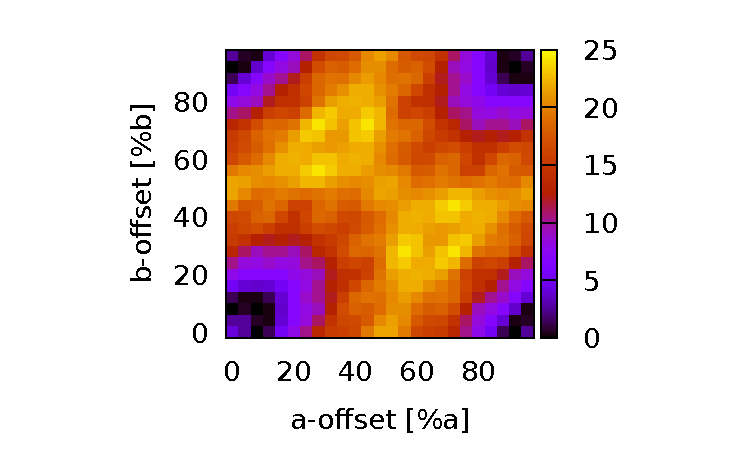
\includegraphics[trim={2cm 0cm 1.9cm 0.4cm},clip,width=8.5cm]{images/DFTB_all_05000N2_map.pdf}} \\ 
\multicolumn{2}{c}{\textbf{\Large{DFTB+}}\par\medskip}\\
\end{tabular}}
\caption{Mapping of the offset-dependent potential for COF 05000N2; for every x-y point, only the z-value leading to the lowest energy was kept; energy in $kcal/mol$}
\label{fig:50maps}
\end{figure}






\begin{figure}[H]
\vspace{2cm}
\begin{centering}
\textbf{\LARGE{05001N2}}\par\medskip
\end{centering}
\makebox[\textwidth][c]{
\begin{tabular}{cc}
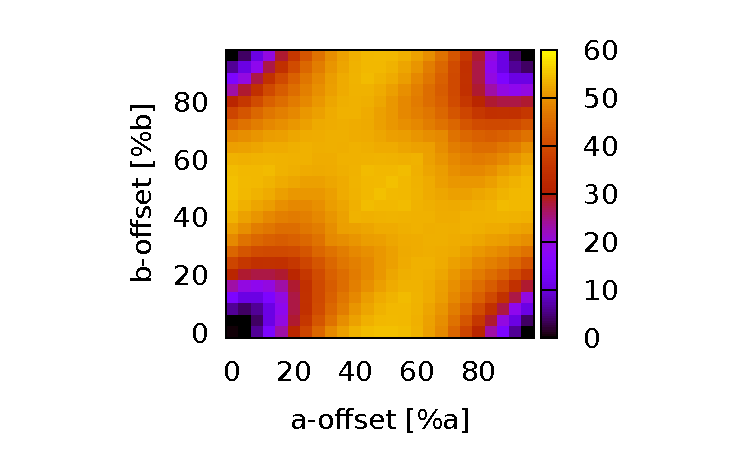
\includegraphics[trim={2cm 0cm 1.9cm 0.4cm},clip,width=8.5cm]{images/LJ_all_05001N2_map.pdf}& 
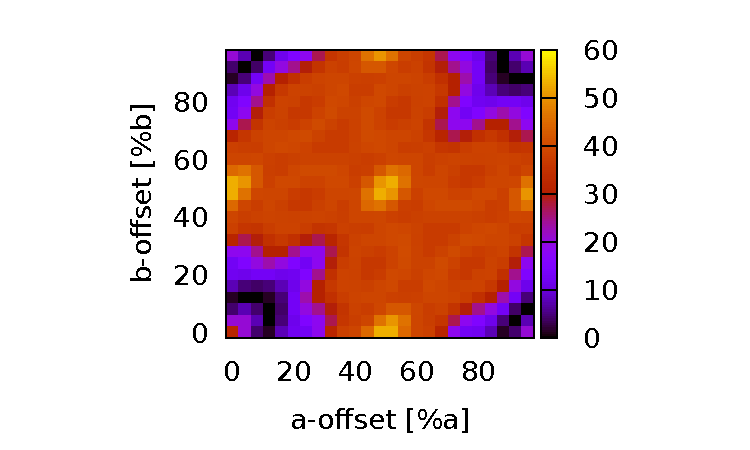
\includegraphics[trim={2cm 0cm 1.9cm 0.4cm},clip,width=8.5cm]{images/LAMMPS_all_05001N2_map.pdf}\\
\textbf{\Large{LJ}}\par\medskip & \textbf{\Large{LJ+Coul.}}\par\medskip\\
\multicolumn{2}{c}{ 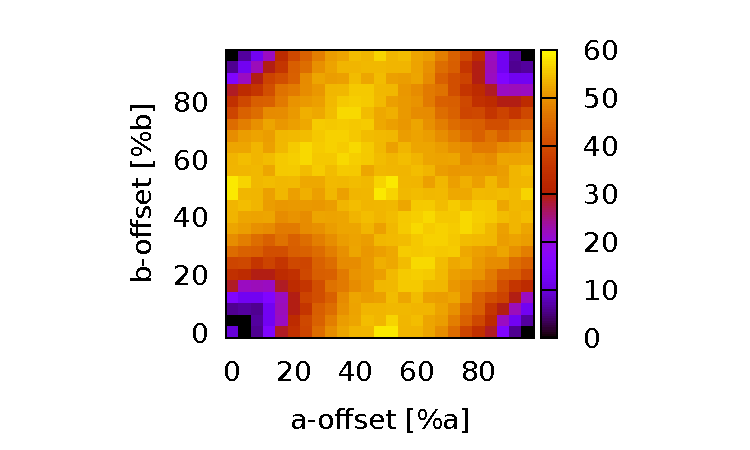
\includegraphics[trim={2cm 0cm 1.9cm 0.4cm},clip,width=8.5cm]{images/DFTB_all_05001N2_map.pdf}} \\ 
\multicolumn{2}{c}{ \textbf{\Large{DFTB+}}\par\medskip}\\
\end{tabular}}
\caption{Mapping of the offset-dependent potential for COF 05001N2; for every x-y point, only the z-value leading to the lowest energy was kept; energy in $kcal/mol$}
\label{fig:51maps}
\end{figure}







\begin{figure}[H]
\vspace{2cm}
\begin{centering}
\textbf{\LARGE{10000N2}}\par\medskip
\end{centering}
\makebox[\textwidth][c]{
\begin{tabular}{cc}
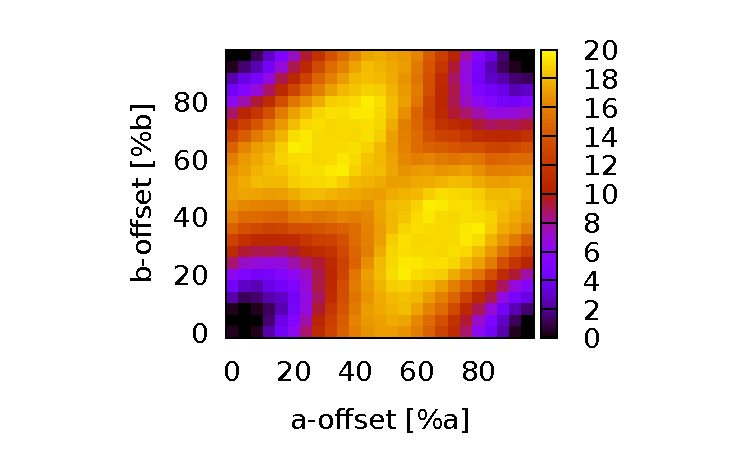
\includegraphics[trim={2cm 0cm 1.9cm 0.4cm},clip,width=8.5cm]{images/LJ_all_10000N2_map.pdf}& 
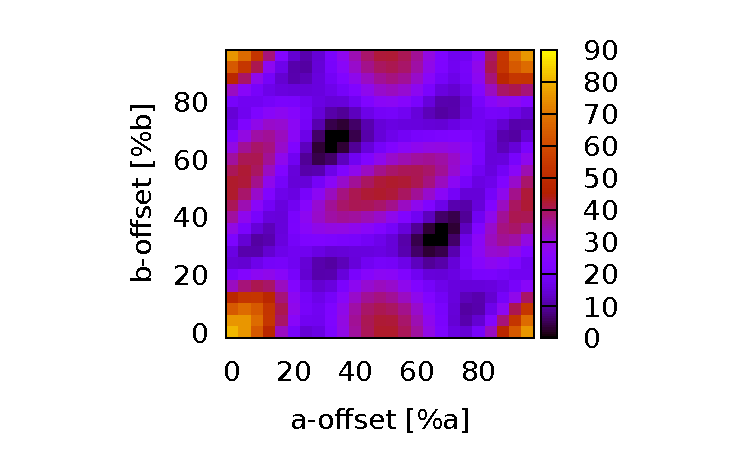
\includegraphics[trim={2cm 0cm 1.9cm 0.4cm},clip,width=8.5cm]{images/LAMMPS_all_10000N2_map.pdf}\\
\textbf{\Large{LJ}}\par\medskip & \textbf{\Large{LJ+Coul.}}\par\medskip\\
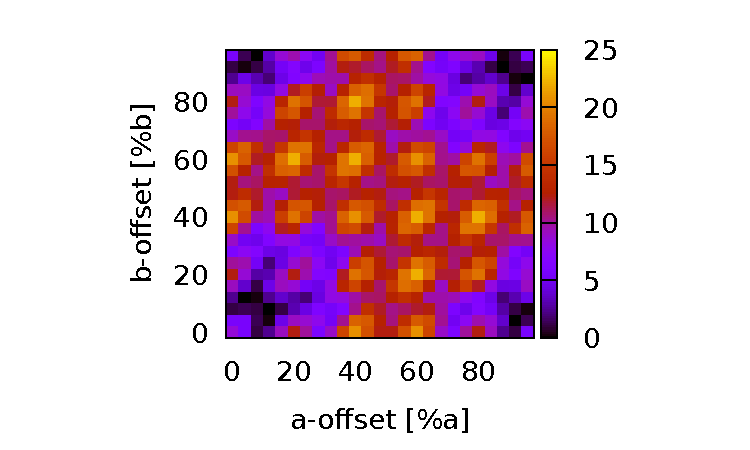
\includegraphics[trim={2cm 0cm 1.9cm 0.4cm},clip,width=8.5cm]{images/xTB_all_10000N2_map.pdf}& 
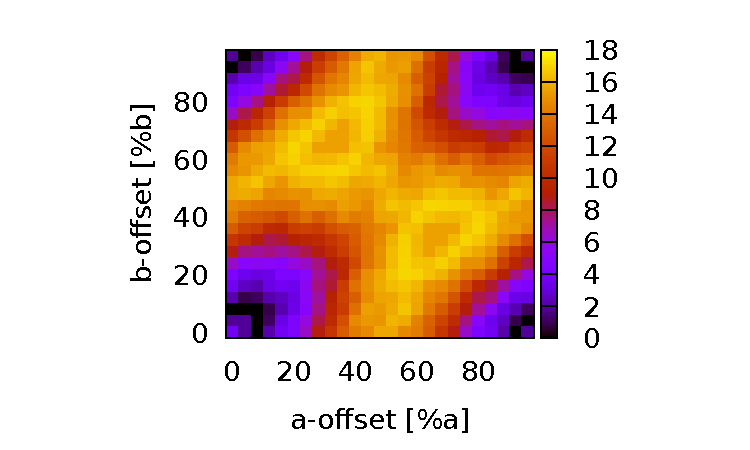
\includegraphics[trim={2cm 0cm 1.9cm 0.4cm},clip,width=8.5cm]{images/DFTB_all_10000N2_map.pdf} \\ 
\textbf{\Large{xTB}}\par\medskip & \textbf{\Large{DFTB+}}\par\medskip\\
\end{tabular}}
\caption{Mapping of the offset-dependent potential for COF 10000N2; for every x-y point, only the z-value leading to the lowest energy was kept; energy in $kcal/mol$}
\label{fig:10maps}
\end{figure}



\begin{figure}[H]
\vspace{2cm}
\begin{centering}
\textbf{\LARGE{13000N2}}\par\medskip
\end{centering}
\makebox[\textwidth][c]{
\begin{tabular}{cc}
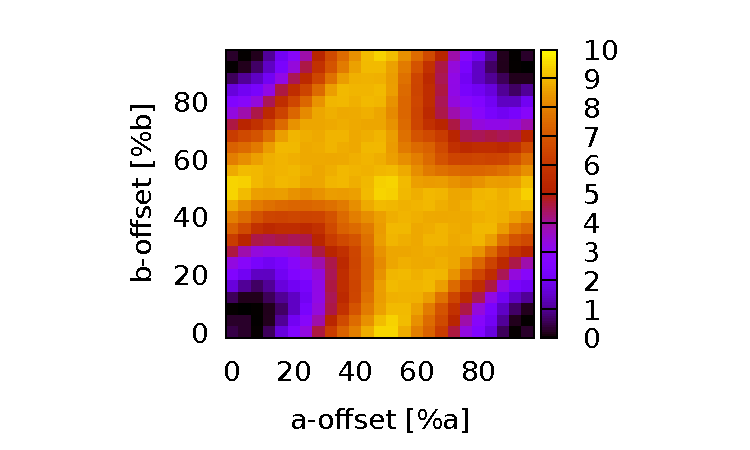
\includegraphics[trim={2cm 0cm 1.9cm 0.4cm},clip,width=8.5cm]{images/LJ_all_13000N2_map.pdf}& 
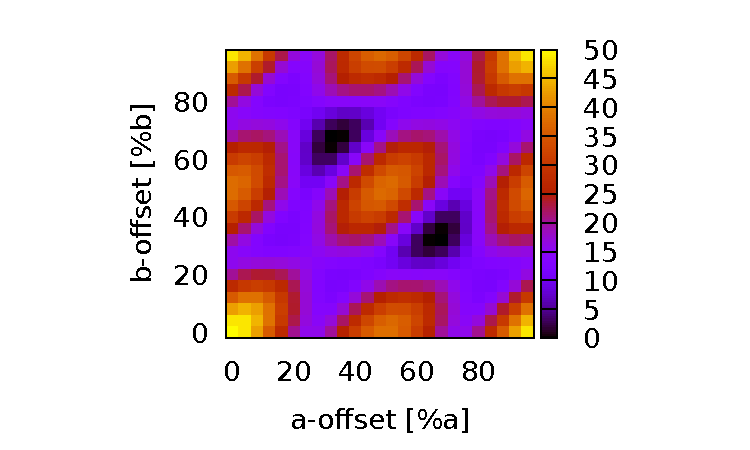
\includegraphics[trim={2cm 0cm 1.9cm 0.4cm},clip,width=8.5cm]{images/LAMMPS_all_13000N2_map.pdf}\\
\textbf{\Large{LJ}}\par\medskip & \textbf{\Large{LJ+Coul.}}\par\medskip\\
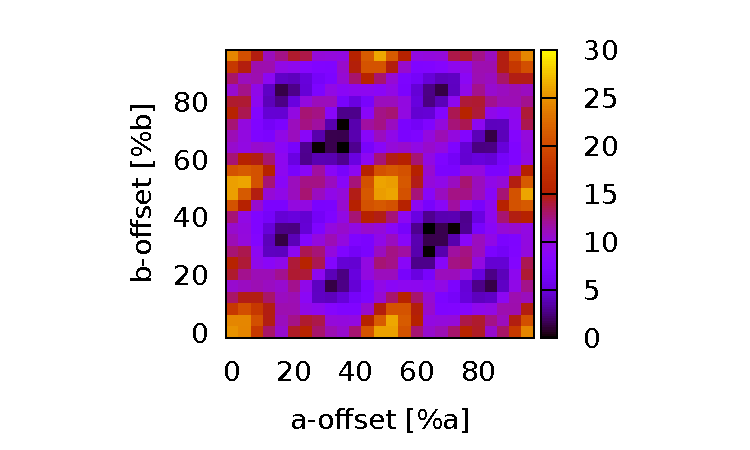
\includegraphics[trim={2cm 0cm 1.9cm 0.4cm},clip,width=8.5cm]{images/xTB_all_13000N2_map.pdf}& 
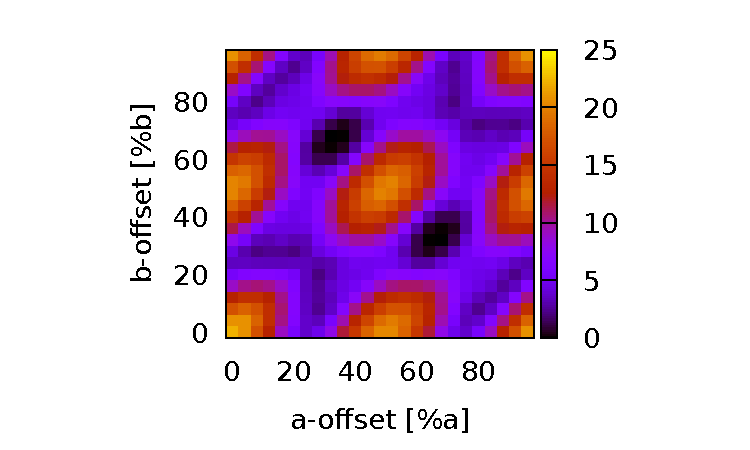
\includegraphics[trim={2cm 0cm 1.9cm 0.4cm},clip,width=8.5cm]{images/DFTB_all_13000N2_map.pdf} \\ 
\textbf{\Large{xTB}}\par\medskip & \textbf{\Large{DFTB+}}\par\medskip\\
\end{tabular}}
\caption{Mapping of the offset-dependent potential for COF 13000N2; for every x-y point, only the z-value leading to the lowest energy was kept; energy in $kcal/mol$}
\label{fig:13maps}
\end{figure}




\begin{figure}[H]
\vspace{2cm}
\begin{centering}
\textbf{\LARGE{17120N2}}\par\medskip
\end{centering}
\makebox[\textwidth][c]{
\begin{tabular}{cc}
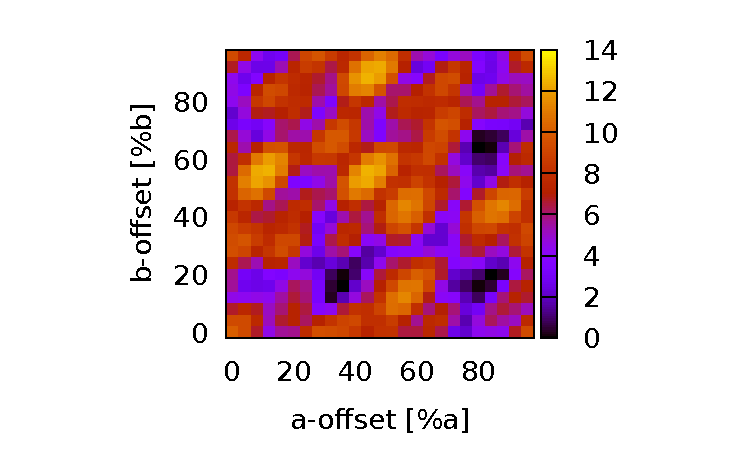
\includegraphics[trim={2cm 0cm 1.9cm 0.4cm},clip,width=8.5cm]{images/LJ_all_17120N2_map.pdf}& 
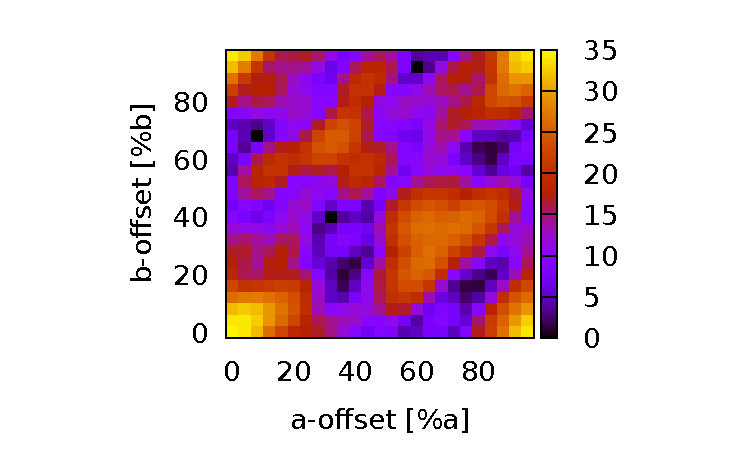
\includegraphics[trim={2cm 0cm 1.9cm 0.4cm},clip,width=8.5cm]{images/LAMMPS_all_17120N2_map.pdf}\\
\textbf{\Large{LJ}}\par\medskip & \textbf{\Large{LJ+Coul.}}\par\medskip\\
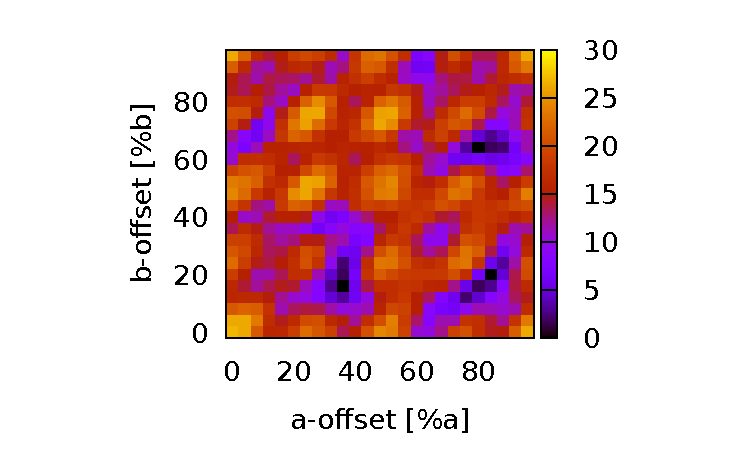
\includegraphics[trim={2cm 0cm 1.9cm 0.4cm},clip,width=8.5cm]{images/xTB_all_17120N2_map.pdf}& 
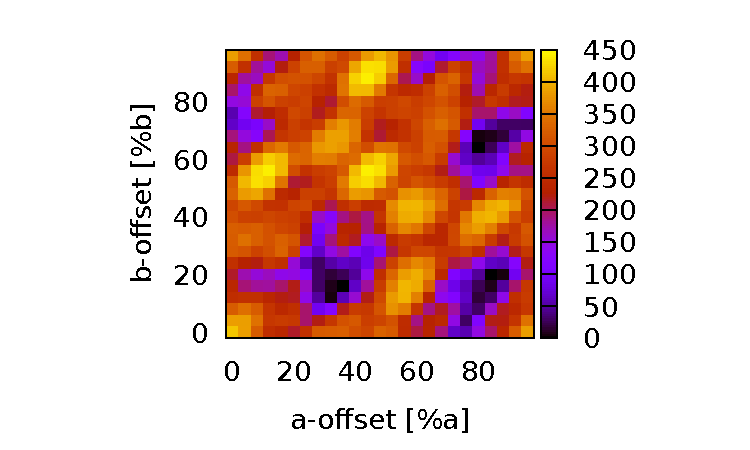
\includegraphics[trim={2cm 0cm 1.9cm 0.4cm},clip,width=8.5cm]{images/DFTB_all_17120N2_map.pdf} \\ 
\textbf{\Large{xTB}}\par\medskip & \textbf{\Large{DFTB+}}\par\medskip\\
\end{tabular}}
\caption{Mapping of the offset-dependent potential for COF 17120N2; for every x-y point, only the z-value leading to the lowest energy was kept; energy in $kcal/mol$}
\label{fig:17maps}
\end{figure}



\begin{figure}[H]
\vspace{2cm}
\begin{centering}
\textbf{\LARGE{18112N2}}\par\medskip
\end{centering}
\makebox[\textwidth][c]{
\begin{tabular}{cc}
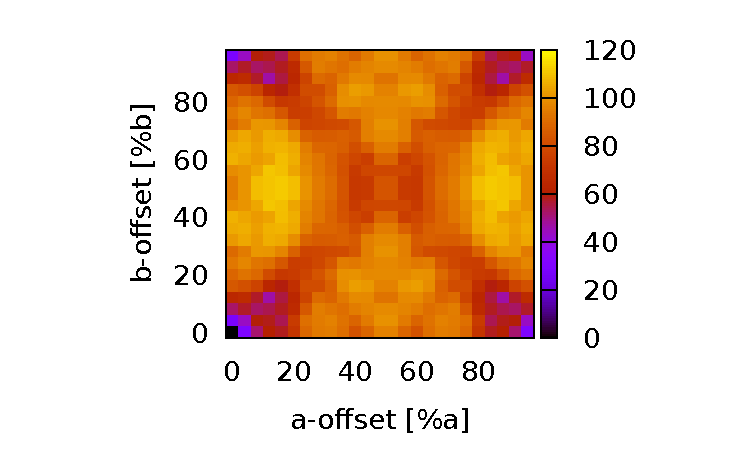
\includegraphics[trim={2cm 0cm 1.9cm 0.4cm},clip,width=8.5cm]{images/LJ_all_18112N2_map.pdf}& 
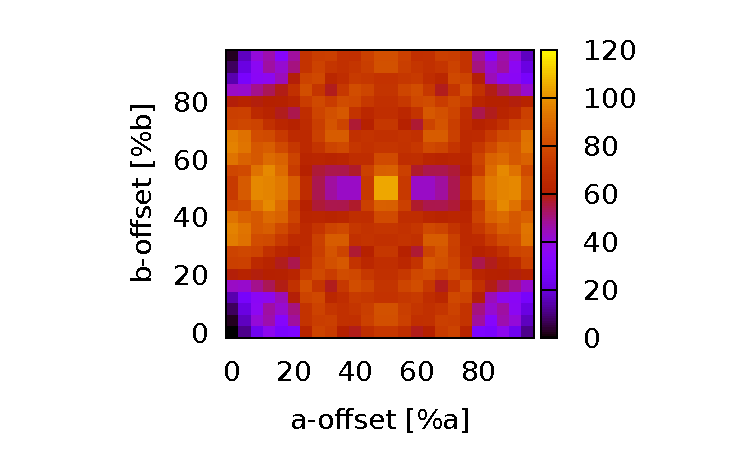
\includegraphics[trim={2cm 0cm 1.9cm 0.4cm},clip,width=8.5cm]{images/LAMMPS_all_18112N2_map.pdf}\\
\textbf{\Large{LJ}}\par\medskip & \textbf{\Large{LJ+Coul.}}\par\medskip\\
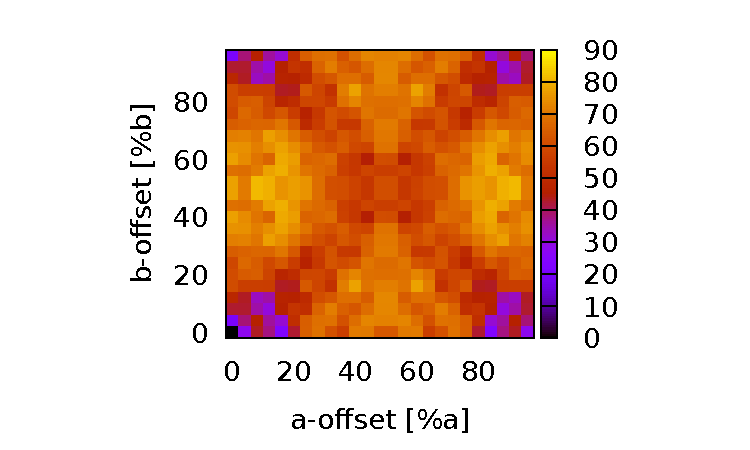
\includegraphics[trim={2cm 0cm 1.9cm 0.4cm},clip,width=8.5cm]{images/xTB_all_18112N2_map.pdf}& 
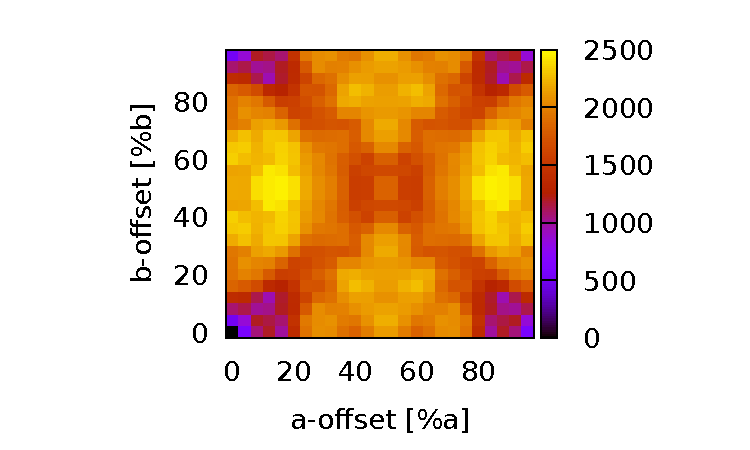
\includegraphics[trim={2cm 0cm 1.9cm 0.4cm},clip,width=8.5cm]{images/DFTB_all_18112N2_map.pdf} \\ 
\textbf{\Large{xTB}}\par\medskip & \textbf{\Large{DFTB+}}\par\medskip\\
\end{tabular}}
\caption{Mapping of the offset-dependent potential for COF 18112N2; for every x-y point, only the z-value leading to the lowest energy was kept; energy in $kcal/mol$}
\label{fig:18maps}
\end{figure}



\subsection{Limitations of CP2K xTB}
\label{sec:xTB_fail}
The implementation of xTB used in this project was the development version implemented on CP2K. Bugs were reported to us over the course of the project that explains the long runtime that was observed and could explain the regular grid-like pattern that appears on the PES. Because of the unstability of this program, the calculations using this method were abandoned over the course of the project. Nonetheless it would be interesting to re-iterate the experiment when a stable version of this program will be available.

\subsection{Influence of initial structure}

\subsection{Influence of point charge assignment method}

A crucial point in estimating the classical Coulombic interactions is the assignment of point-charges. Different methods were tested for that purpose. As a first estimation the EGULP charge equilibration routine was tested. The table below displays (see Figure \ref{fig:symetry}) the charge distribution over atoms and their mirror image along the a=b plane in the symmetric COF 13000N2. The charge distribution is compared to the Hirshfeld charges obtained using DFT. As one can see on the table below the charge repartition is strongly asymetric, which is an unphysical behavior (since a symmetric molecule must lead to an electron density having at least the same symmetries)
Furthermore some benzene-bounded Fluorine have positive point charges which, given the electron-donating abilities of benzene and the very strong electronegativity of Fluorine is unlikely. Hirshfeld point charge partition, although not perfectly symmetric, yield a much more reasonable charge repartition.
The asymetry could be caused by the very slight deviations to a perfect symmetry in the COF structure (>$10^{-3}\AA$). Indeed these are too slight to justify the  deviations observed with EGULP but could explain the ones observed with DFT.

%
\begin{figure}[H]
\begin{centering}
\textbf{Charge symmetry comparison}\par\medskip
\scalebox{0.7}{
\begin{tabular}{|c||c|c||c|c|}
\hline
Element & \multicolumn{2}{c||}{Egulp} &\multicolumn{2}{c|}{Hirshfeld}\\
\hline
\hline
C&0.325&0.414&0.275&0.275\\
\hline
C&0.201&0.08&0.009&0.009\\
\hline
C&0.324&0.423&0.276&0.275\\
\hline
C&0.205&0.088&0.009&0.009\\
\hline
C&0.417&0.375&0.309&0.309\\
\hline
F&-0.466&-0.432&-0.306&-0.304\\
\hline
C&0.49&0.505&0.311&0.31\\
\hline
F&-0.37&0.107&-0.312&-0.301\\
\hline
C&0.065&-0.296&0.308&0.307\\
\hline
F&-0.511&-0.48&-0.314&-0.305\\
\hline
C&0.418&0.376&0.31&0.309\\
\hline
F&-0.465&-0.437&-0.306&-0.306\\
\hline
C&0.492&0.49&0.311&0.307\\
\hline
F&-0.37&0.114&-0.309&-0.312\\
\hline
C&0.062&-0.304&0.31&0.307\\
\hline
F&-0.517&-0.479&-0.302&-0.305\\
\hline
N&-0.328&-0.179&-0.287&-0.279\\
\hline
N&-0.327&-0.186&-0.287&-0.287\\
\hline
\end{tabular}
}
\caption{Comparison of the symmetry of charge repartitions using different charge equilibration method for the symmetric COF 13000N2; every atom's charge is compared to its mirror image along the symmetry axis for each technique}
\label{fig:symetry}
\end{centering}
\end{figure}

\subsection{Influence of the stacking on the electronic structure}

The equilibrium electronic structure of a molecule is influenced by the electrical field surrounding it. Since COFs are polarized, they create an electrical field which, at short distance, could influence the electronic structure of the adjacent layers. In order to assess the need to equilibrate the charge density, for every stacking configuration, the Hirshfeld as computed by DFTB+ for every grid-point were compared for a subset of COFs. Key statistical values of this analysis are displayed on the table below (see Figure \ref{fig:chg_var}).

\begin{figure}[H]
\begin{centering}
\textbf{Charge variation analysis}\par\medskip
\scalebox{0.7}{
\begin{tabular}{|c||c|c|}
\hline
COF&$max(\Delta(Q(x,y,z)))$ &$\overline{\sigma(Q_i(x,y,z)}$\\
\hline
\hline
05000N2&0.372&0.03958\\
\hline
05001N2&0.275&0.01922\\
\hline
10000N2&0.438&0.04028\\
\hline
13000N2&0.403&0.11313\\
\hline
17120N2&0.612&0.04851\\
\hline
\end{tabular}
}
\caption{analysis of the changes in charge partition as a function of the offset where $max(\Delta(Q(x,y,z)))$ is the maximum observed difference of charge for a given element and $\overline{\sigma(Q(x,y,z)}$ is the average over all elements of the standard deviation computed for each element in the COF}
\label{fig:chg_var}
\end{centering}
\end{figure}